\documentclass{article}
\usepackage[utf8]{inputenc}
\usepackage{graphicx}
\usepackage{mathtools}
\usepackage{float}

\title{B-Spline Curvature Extrema}
\author{davidc}
\date{July 2022}

\begin{document}

\maketitle

\section{Introduction}

Curvature constrained paths are used in various computer aided applications such as computer graphics, highway design, trajectory generation, and data estimation. Some traditional methods like the Markov-Dubins method use straight lines and arcs to generate paths \cite{ARTICLE:Hota}. More recent work combines arcs with monotonic Bezier curves \cite{ARTICLE:Wang}. Paths that use splines such as Bezier or B-spline curves are desirable because their bounds and location can be constrained through their control points. However most methods that rely only on spline curves bound the curvature by evaluating the curvature at discrete locations along the curve \cite{ARTICLE:Cimurs}, \cite{ARTICLE:Kano}. Other spline methods that create bounds from the control point geometry are limited to two dimensions \cite{ARTICLE:Walton}\cite{ARTICLE:Walton2}, or work only for second degree splines \cite{ARTICLE:Deddi}.

This paper seeks the optimal method of generating B-spline paths in three dimensions and for any spline degree. It compares various approaches for constraining the curvatures of a B-spline with varying degrees of speed, accuracy, and conservativeness. The objective in the first set of tests is to find the maximum curvature of a B-spline in a given knot-point interval. The goal for the second set of tests is to generate a curvature constrained path of minimum length between two waypoints each with a direction vector.

\section{Preliminaries}


\begin{itemize}
  \item[] b(t) = B-spline curve
  \item[] k = order or degree of the polynomial.
  \item[] n \(=\) number of control points.
  \item[] \(P_i = i^{th}\) control point.
  \item[] m = number of knot points.
  \item[] \(\mu\) = number of knot intervals.
  \item[] \(t_i = i^{th}\) knot point.
  \item[] \(N_{i , \textbf{k}}\) = \(i^{th}\) basis function of a \textbf{k} degree B-spline.
  \item[] \(\alpha\) = spacing between uniform knot points
  \item[] C(t) = curvature function
  \item[] \(\nu\) = b(t)' = velocity
  \item[] a = b(t)'' = acceleration
  \item[] B(t) = Bezier curve
  \item[] \(\beta_i = i^{th}\) Bezier control point.
  \item[] \(\rho_{i , \textbf{k}}\) = \(i^{th}\) Bernstein basis polynomial of a \textbf{k} degree Bezier curve.
\end{itemize}

\subsection{B-Splines}

\begin{figure}[H]
\begin{center}
\includegraphics[scale=.5]{2ndOrderBspline.png}
\end{center}
\caption{Second order Open Uniform B-spline}
\label{Fig:2ndOrderBspline}
\end{figure}

 A B-spline or \say{basis spline} is a piece-wise polynomial function of degree k. The formal definition for a b-spline is given by the following equation.
 
   \begin{equation} \label{eq:B-Spline equation}
      b(t) = \sum^{n-1}_{i=0} N_{i,k}(t) P_i
  \end{equation}
  
  Here, k is the order or degree of the spline, and \(n\) is the number of control points. \(P_i\) and \(N_{i,k}(t)\) is the \(i^{th}\) control point and basis function respectively. \(N_{i,k}(t)\) can be evaluated using the Cox-de-boor recursion formula. We note that the B-spline is defined only between the knot points \(t_k\) and \(t_n\), where each interval \([t_i , t_{i+1})\) describes one of the polynomials that make up the B-spline.

\begin{equation}
    \Big[ t_0, \; t_1,  \; ... \; t_{k-1} , \; \underbrace{t_k, \; t_{k+1}, \; ... \; t_n,}_{\text{defined}} \; t_{m-k}, \; t_{m-k+1}, \; ... \; t_{m-1} \Big]
\end{equation}
  
  We can also define B-splines using the matrix form.
  
\begin{equation}
\begin{aligned}
        b(t) & = \textbf{P}_i M L \\
           b(t) & = \begin{bmatrix} P_{i} & P_{i+1} & ... & P_{i+k}\end{bmatrix} M \begin{bmatrix} (\frac{t-t_j}{\alpha})^k \\ \\ ... \\ \\ (\frac{t-t_j}{\alpha})^2 \\ \\ (\frac{t-t_j}{\alpha}) \\ \\ 1 \end{bmatrix}
\end{aligned}
\end{equation}

for 

    \begin{equation}
        t_j \leq t < t_{j+1} \quad , \quad i = j-k \quad , \quad \alpha = t_{i+1} - t_i
    \end{equation}

\(M\) is the multiplier matrix specific to the order of the B-spline. See the appendix for details.

\subsection{Bezier Curves}
    Some of the methods described in this paper use the Bezier curve representation for individual knot intervals of the B-spline. A Bezier curve is a parametric curve or polynomial of degree k, that is defined between the interval \([t_0, t_0 + \alpha]\). A set of discrete control points \(\boldsymbol{\beta}\) shapes the curve. The Bernstein formula that defines a Bezier curve is shown below.

\begin{equation}
    B(t) = \sum_{i=0}^{\textbf{k}}\beta_i \;\rho_{i,\textbf{k}}(t)
\end{equation}

for

\begin{equation}
    t_0 \leq t \leq (t_0 + \alpha)
\end{equation}

\begin{equation}
    \boldsymbol{\beta} = [\beta_0, \beta_i, ... \beta_{\textbf{k}}]
\end{equation}

\begin{equation}
    \rho_{i,\textbf{k}}(t) = \binom{\textbf{k}}{i}(1 - \tau)^{\textbf{k}-i}\;\tau^i
\end{equation}

\begin{equation}
    \tau = \frac{t-t_0}{\alpha}
\end{equation}
    
\begin{figure}[H]
\begin{center}
\includegraphics[scale=.2]{BsplineToBezier.png}
\end{center}
\caption{Set of B-spline control points converted to Bezier control points.}
\label{Fig:BsplineToBezier}
\end{figure}

The equation to transform a set of B-spline control points to Bezier control points are as follows.

\begin{equation}
    \boldsymbol{\beta} = \textbf{P}_i F
\end{equation}

or

\begin{equation}
    [\beta_0, \beta_1, ... \beta_{\textbf{k}}] = [P_i, P_{i+1}, ... P_{i+\textbf{k}}] F
\end{equation}

Where F is a transformation matrix. See the appendix for the the values of the F matrix.

\subsection{Curvature}

The curvature at specific point is defined by the circle that best approximates the shape of the curve at that point. It is formally defined by the inverse radius of the circle. See figure \ref{Fig:Curvature}. 

\begin{figure}[h]
\begin{center}
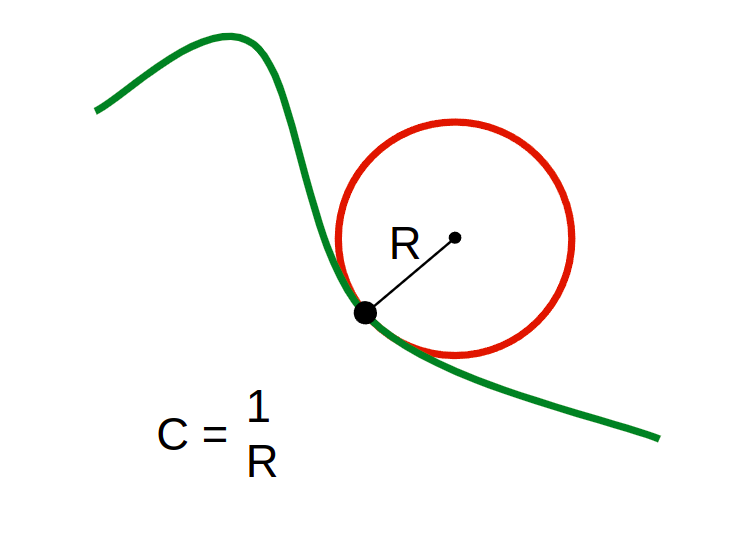
\includegraphics[scale=.23]{Curvature.png}
\end{center}
\caption{Curvature defined by the oscillating circle}
\label{Fig:Curvature}
\end{figure}

The curvature of a B-spline \(b(t)\) with first and second derivatives \(b(t)'\) and \(b(t)''\) is defined as follows.

\begin{equation} \label{eq:curvature}
    C(t) = \frac{||b_{(t)}' \times b_{(t)}''||}{||b_{(t)}'||^3}
\end{equation}

Using the rules for the derivative of a cross product and the derivative of a norm, we can show the derivative of the curvature. We also use the third derivative of the spline \(b(t)'''\). See appendix for derivative rules.

\begin{equation}
    C(t)' = \frac{(b_{(t)}' \times b_{(t)}'') \cdot (b_{(t)}' \times b_{(t)}''')}{||b_{(t)}' \times b_{(t)}''||\;||b_{(t)}'||^3} - \frac{3(b_{(t)}' \cdot b_{(t)}'') || b_{(t)}' \times b_{(t)}''||}{||b_{(t)}'||^5}
\end{equation}


We can also define the curvature with the portion of the second derivative that is perpendicular to the first derivative. This relation comes from the equation for centripetal acceleration. See Figure (\ref{Fig:Centripetal_Acceleration}).


\begin{figure}[h]
\begin{center}
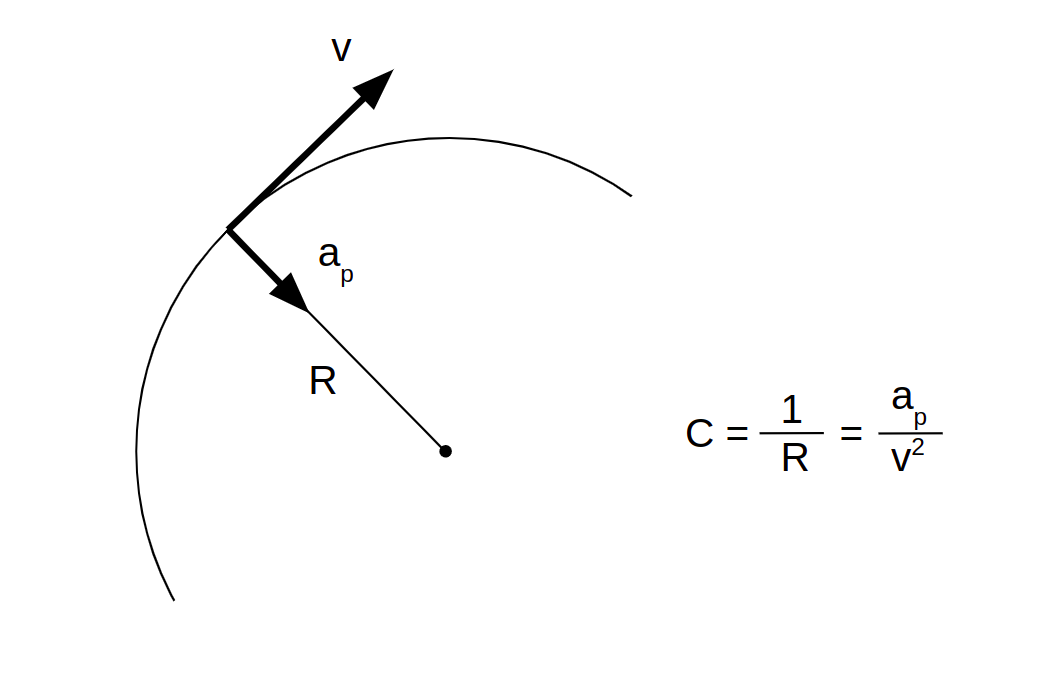
\includegraphics[scale=.23]{Centripetal_Acceleration.png}
\end{center}
\caption{Centripetal Acceleration Equation}
\label{Fig:Centripetal_Acceleration}
\end{figure}

\begin{equation} \label{eq:curvature using centripetal}
    C(t) = \frac{||b_{(t)}_p''||}{||b_{(t)}'||^2}
\end{equation}

where the perpendicular portion of the second derivative is equal to the following.

\begin{equation}
\begin{aligned}
    b(t)_p'' &= b(t)'' -  \Bigl(b(t)' \cdot b(t)''\Bigl) \frac{b(t)'}{||b(t)'||^2} \\
    &= \frac{||b(t)' \times b(t)''||} {||b(t)'||}
\end{aligned}
\end{equation}

\subsection{Objectives}

\subsubsection{First Objective}

The objective in these series of tests is to find the maximum curvature over a single knot point interval of a B-spline, while testing the speed, accuracy and conservatives of each method to find the max curvature.

\begin{equation}
    \text{Find} \quad C(t)_{max} \quad \text{for} \quad t \in [t_j,t_{j+1}]
\end{equation}

For simplicity we will assume that the number of control points \(n\) is equal to \(k + 1\), the order of the spline plus one. This means that the spline has only one knot interval. If we also assume that the scale factor \(\alpha\) is equal to unity, then we get following objective.

\begin{equation}
    \text{Find} \quad C(t)_{max} \quad \text{for} \quad t \in [0,1]
\end{equation}

where

   \begin{equation} \label{eq:B-Spline equation}
      b(t) = \sum^{k}_{i=0} N_{i,k}(t) P_i
  \end{equation}
  
  or
  
  \begin{equation}
    b(t) = \begin{bmatrix} P_{0} & P_{1} & ... & P_{k}\end{bmatrix} M \begin{bmatrix} t^k \\ \\ ... \\ \\ t^2 \\ \\ t \\ \\ 1 \end{bmatrix}
\end{equation}

\subsubsection{Second Objective}

The objective in these series of tests is to generate an optimal path between two waypoints with directional vectors, while comparing the speed of the path generation, accuracy of the curvature constraint, and length of the paths for each curvature bounding method.

\section{Methods for Estimating Curvature Extrema}
\subsection{Maximizing the Curvature Equation}

In this method we will maximize the objective function for curvature. Or minimize the negative curvature.

\begin{equation}
\begin{aligned}
    \text{minimize} & \quad -C(t) \\
    \text{by varying} & \quad t \in [0,1] \\
    \text{with Jacobian} & \quad -C(t)' 
\end{aligned}
\end{equation}

Here we use the Sequential Quadratic Programming approach to perform the optimization. Specifically "the Han–Powell quasi–Newton method with a BFGS update of the B–matrix and an L1–test function in the step–length algorithm". In order to find a global maximum, the optimization is performed over k+1 initial conditions spread out evenly over the knot interval.

\begin{equation}
    t_{initial} = (0, \frac{1}{k}, \frac{2}{k} ... 1) 
\end{equation}

Figure \ref{Maximum Curvature} shows the optimization performed on the curvature of the example 3rd order B-spline.

\begin{figure}[H]
\centering
\includegraphics[scale=.5]{MaximumCurvatureEquation.png}
\caption{Finding max curvature using SQP approach}
\label{Maximum Curvature}
\end{figure}

The average accuracy for this method is 100 percent and the average time it takes for this method is 0.003 sec.

\subsection{Roots of the Curvature Derivative}

In this method we use the Brent–Dekker method to find the roots of the curvature derivative.

\begin{equation}
\begin{aligned}
    \text{roots of} & \quad C(t)' = 0 \\
    \text{bounded by} & \quad t \in [0,1] \\
\end{aligned}
\end{equation}

Again, since we are searching for a global maximum curvature, we split up the intervals for which we perform a root search into \(k + 2\) intervals or brackets. Figure \ref{RootsCurvatureDerivative} shows this root finding method performed over the curvature derivative of the example 3rd order B-spline, over four bracket intervals.

\begin{figure}[H]
\centering
\includegraphics[scale=.2]{RootsCurvatureDerivative.png}
\caption{Finding roots of curvature derivative using Brent-Decker method}
\label{RootsCurvatureDerivative}
\end{figure}

The average accuracy for this method is 99 percent and the average time is 0.002 sec.

\subsection{Discrete Evaluations}
This method involves finding the curvature at \(\eta\) points along the spline interval. Accuracy increase with \(\eta\), but so does time. 

\begin{figure}[H]
\begin{center}
\includegraphics[scale=.6]{CurvatureAtNPoints.png}
\end{center}
\caption{Curvature at N discrete points}
\label{Fig:CurvatureAtNPoints}
\end{figure}

If we set up the evaluation in matrix form, we can evaluation of all the points in a knot interval with a few equations. First we evaluate the first and second derivative of the B-spline (b(t)' and b(t)''). Here (r) is the derivative order.



\begin{equation}
\begin{aligned}
    b(t_i \rightarrow t_{i+1}) &= \textbf{P}_i M \textbf{K}\textbf{L}_r\\
    b(t_i \rightarrow t_{i+1}) &= \begin{bmatrix} P_i, & P_{i+1}, & ... & P_{i+\textbf{k}} \end{bmatrix} M \textbf{K} \begin{bmatrix} 0 & \delta^{\textbf{k}-r} & (2\delta)^{\textbf{k}-r}& ... & \big((\eta-1) \delta\big)^{\textbf{k}-r}\\
    & ... & & & ... \\ \\
    0^2 &  \delta^2 & (2\delta)^2 & ... & \big((\eta-1) \delta\big)^2 \\ 
     0 &  \delta & 2\delta & ... & (\eta-1) \delta \\ 
     1 & 1 & 1 & ... & 1 \\
     \textbf{0}_{r \times 1} & \textbf{0}_{r \times 1} & \textbf{0}_{r \times 1} & ... & \textbf{0}_{r \times 1}\end{bmatrix}_{\in \mathbb{R}^{\textbf{k}+1 \times \eta}}
\end{aligned}
\end{equation}

where

\begin{equation}
    \delta = \frac{1}{\eta-1}
\end{equation}

\begin{equation}
    \textbf{K} = \frac{1}{\alpha^r}\begin{bmatrix} \frac{\textbf{k}!}{(\textbf{k}-r)!} & & & &  \textbf{0}\\ 
    & ... & & & & 
    \\ 
    & &  \frac{(r+1)!}{1!} & &
    \\  & & & \frac{(r)!}{0!} &
    \\ \textbf{0} &  & & & \textbf{0}_{r \times r} \end{bmatrix}_{\in \mathbb{R}^{\textbf{k}+1 \times \textbf{k}+1}}
\end{equation}

\begin{equation}
    b(t_j \rightarrow t_{j+1}) \in \mathbb{R}^{d \times \eta}, \quad i = j-\textbf{k}
\end{equation}

We can then perform vector math operations to evaluate the curvature for the knot interval.

\begin{equation}
    C(t) = \frac{||b(t_j \rightarrow t_{j+1})' \times b(t_j \rightarrow t_{j+1})''||}{||b(t_j \rightarrow t_{j+1})'||^3}
\end{equation}

\subsection{Curvature at the Minimum Velocity} \label{Curvature at Min Velocity}

Looking at the equation for curvature (\ref{eq:curvature});

\begin{equation}
    C(t) = \frac{||b_{(t)}' \times b_{(t)}''||}{||b_{(t)}'||^3}
\end{equation}

We can see that the maximum curvature will most likely occur near the minimum velocity. This is true for splines up to the third order. Figure \ref{Time at minimum velocity and maximum curvature} shows this property for a 2nd and 3rd order B-spline. 

\begin{figure}[H]
\centering
\includegraphics[scale=.28]{CurvatureAtMinimumVelocity.png}
\caption{CurvatureAtMinimumVelocity}
\label{Time at minimum velocity and maximum curvature}
\end{figure}

\subsubsection{Minimum Velocity}

To find the min velocity we must find the roots of the derivative of the velocity magnitude.

\begin{equation}
    \frac{d ||b(t)'||}{dt} = \frac{b(t)' \cdot b(t)''}{||b(t)'||} = 0
\end{equation}

or the roots of;

\begin{equation} \label{eq:roots of velocity derivative}
    b(t)' \cdot b(t)'' = 0
\end{equation}

We can express this in Matrix form as follows.

\begin{equation} \label{velocity derivative}
    L'^T M^{T}\textbf{P}_i^{T}\textbf{P}_iML'' = 0
\end{equation}

where 

\begin{equation}
    L'=\begin{bmatrix} kt^{k-1} \\ ... \\ 3t^2 \\ 2t \\ 1 \\ 0 \end{bmatrix} \quad L''=\begin{bmatrix} k(k-1)t^{k-2} \\ ... \\ 6t \\ 2 \\ 0 \\ 0 \end{bmatrix}
\end{equation}

This results in a third order polynomial for 3rd order splines, and a 1st order polynomial for second order splines. Each of which we can find the roots for in linear time. If us define the middle terms of equation (\ref{velocity derivative}), we can express it in polynomial form.

\begin{equation}
    J = M^{T}\textbf{P}_i^{T}\textbf{P}_iM
\end{equation}

\hspace{1cm}

\textbf{Second Order Spline}

\hspace{1cm}

\begin{equation}
    b(t)' \cdot b(t)'' = 8J_{11}\textbf{t} + 4J_{21}
\end{equation}

where

\begin{equation}
    J = M^{T}\textbf{P}_i^{T}\textbf{P}_iM = \begin{bmatrix} J_{11} & J_{12} & J_{13} \\
                        J_{21} & J_{22} & J_{23} \\
                        J_{31} & J_{32} & J_{33} \end{bmatrix}
\end{equation}  

\hspace{1cm}

\textbf{Third Order Spline}

\hspace{1cm}

\begin{equation}
     b(t)' \cdot b(t)'' =  36J_{11}\textbf{t}^3 + (12J_{12} + 24J_{21})\textbf{t}^2 + (8J_{22} + 12J_{31})\textbf{t} + 4J_{32}
\end{equation}

where

\begin{equation}
    J = M^{T}\textbf{P}_i^{T}\textbf{P}_iM = \begin{bmatrix} J_{11} & J_{12} & J_{13} & J_{14} \\
                        J_{21} & J_{22} & J_{23} & J_{24} \\
                        J_{31} & J_{32} & J_{33} & J_{34} \\
                        J_{41} & J_{42} & J_{43} & J_{44}\end{bmatrix}
\end{equation}  

\hspace{1cm}

\textbf{Roots}

\hspace{1cm}

To find the roots of \(b(t)' \cdot b(t)''\) for a second order spline we can use the the quadratic formula. For a third order spline we must use some form of Cardano's formula. See \cite{WEBPAGE:Weisstein} for the process of finding the roots of a cubic equation.

The minimum velocity will exist at one of the roots.

\subsubsection{Max Curvature at Roots}

The maximum curvature in the interval will exist close to a root, or the start or end point of the knot-interval. This is valid because the maximum acceleration is always at the beginning or end of the interval for a second and third order spline because the equation for the acceleration magnitude is linear for a quadratic spline, and quadratic for a cubic spline. 

 After the curvature is evaluated at each root and endpoint, the last step is to choose the max out of each evaluation.

\begin{equation}
    C(t)_{\text{max} \; \text{est}} = \text{max}\{C(t_j),\; C(t_{j+1}), \; C(t_{r1}),\; ... ,C(t{r_i})\} 
\end{equation}

where i is the number of roots within the interval \([t_j , t_{j+1}]\).

\subsection{Bound from Max Cross-Term/Min Velocity}

The curvature can be bounded using the minimum velocity and maximum cross term within a knot interval. 

\begin{equation} 
    C(t) = \frac{||b_{(t)}' \times b_{(t)}''||}{||b_{(t)}'||^3} \leq \frac{\text{max}\{||b_{(t)}' \times b_{(t)}''||\}}{\text{min}\{||b_{(t)}'||\}^3} \quad \text{for} \; t_j \leq t \leq t_{j+1}
\end{equation}

\subsubsection{Minimum Velocity}

The minimum velocity can be found using methods from section \ref{Curvature at Min Velocity}. Once we have found the roots of equation \ref{eq:roots of velocity derivative}, we evaluate the velocity at each root within the knot interval, and at the endpoints of each knot interval. Choose the minimum velocity of those evaluations.

\begin{equation}
    ||b(t)'|| \geq \text{min}\{ ||b(t_j)'|| ,\; ||b(t_{j+1})'|| ,\; ||b(t_{r1})'|| ,\; ... \;  ||b(t_{ri})'|| \}
\end{equation}

where i is number of roots within the interval \([t_j , t_{j+1}]\).

\subsubsection{Maximum Cross-term}

To find the maximum cross-term value we find the roots of the derivative of the cross-term magnitude.

\begin{equation}
    \frac{d||b(t)' \times b(t)''||}{dt} = \frac{\big(b(t)' \times b(t)''\big) \cdot \big(b(t)' \times b(t)'''\big)}{||b(t)' \times b(t)''||} = 0
\end{equation}

or we find

\begin{equation} \label{derivative of cross term}
\begin{aligned}
    \big(b(t)' \times b(t)''\big) \cdot \big(b(t)' \times b(t)'''\big) &= 0 \\
    \big(\textbf{P}_iML' \times \textbf{P}_iML''\big)^{T} \big(\textbf{P}_iML' \times \textbf{P}_iML'''\big) &= 0 
\end{aligned}
\end{equation}

If we evaluate this equation for a second order B-spline, we get zero. If we evaluate for a third order B-spline, we get third order polynomial.

\hspace{1cm}

    \textbf{Cross-term derivative evaluation for a second order spline}
    
\hspace{1cm}

\begin{equation}
    \big(b(t)' \times b(t)''\big) \cdot \big(b(t)' \times b(t)'''\big) = 0
\end{equation}

See section (\ref{sec:Cross-term Derivative Coefficients for a Second Order Spline}) of the appendix for the value of \(||b(t)' \times b(t)''||\).

\hspace{1cm}

    \textbf{Cross-term derivative evaluation for a third order spline}
    
\hspace{1cm}

\begin{equation}
    \big(b(t)' \times b(t)''\big) \cdot \big(b(t)' \times b(t)'''\big) = c_3 t^3 + c_2 t^2 + c_1 t + c_0
\end{equation}

See section (\ref{section:Cross-term Derivative Coefficients for a Third Order Spline}) of the appendix for the values of \(c_i\).

\hspace{1cm}

In polynomial form the roots of ({derivative of cross term}) can be found using either the quadratic formula for second order B-splines, or adaptations of the Cardano formula for third order B-splines (see \cite{WEBPAGE:Weisstein}). Once the roots of equation (\ref{derivative of cross term}) have been found, the cross-term is evaluated at each root, and at the endpoints of each knot interval. The max cross term is the max of these evaluations. For simplicity, the cross term will be called A(t).

\begin{equation}
    A(t) = ||b(t)' \times b(t)''||
\end{equation}

\begin{equation}
    ||A(t)|| \leq \text{max}\{ ||A(t_j)|| ,\; ||A(t_{j+1})|| ,\; ||A(t_{r1})|| ,\; ... \;  ||A(t_{ri})|| \}
\end{equation}

\subsection{Control Point Method}

\subsubsection{Bounds Using Velocity and Acceleration}

Using the the relation between centripetal acceleration and curvature from figure (\ref{Fig:Centripetal_Acceleration}), we can establish bounds on the curvature. Knowing that the total acceleration will always be greater than the centripetal acceleration, the following is true.

\begin{equation} \label{eq:acceleration and velocity bounds}
    C(t) = \frac{a_p(t)}{\nu(t)^2} \leq \frac{a(t)}{\nu(t)^2} 
\end{equation}

The objective is then to bound the minimum velocity, and maximum acceleration in a spline interval.

\subsubsection{Control Point Derivatives}

Using the control point derivatives of a spline, we can bound the max and min values of the spline derivatives. The control point derivatives of a spline are the control points for the new B-spline created when you take the derivative of the spline. Below we show the control point derivative definition for an open B-spline and for a clamped B-spline.

\begin{equation}
\begin{aligned}
    & \textbf{open} \\
    & P_i' = \frac{P_{i+1} - P_{i}}{\alpha}
\end{aligned}
\end{equation}

\begin{equation}
\begin{aligned}
    & \textbf{clamped} \\
    & P_i' = \frac{ P_{i+1} - P_i}{\alpha \; \frac{\text{min}(i+1,\;\mu,\;\textbf{k},\; n-i)}{\textbf{k}}}
\end{aligned}
\end{equation}

\subsubsection{Convex Hull of the Control Points}

Because of the strong convex hull property of B-splines, the spline will always reside within the convex hull of the control points. Therefore the maximum and minimum bounds for a B-spline will be the maximum and minimum of the convex hull. See figure (\ref{Fig:MaxMinBounds}).

\begin{figure}[H]
\begin{tabular}{ll}
\includegraphics[scale=.42]{MaxMinBounds.png}
\end{tabular}
\caption{Maximum and Minimum bounds of a \(3^{rd}\) order B-spline}
\label{Fig:MaxMinBounds}
\end{figure}

\hspace{1cm}

\textbf{Maximum Bound of the Convex Hull}

\hspace{1cm}

 The maximum bound will be the value of the norm of the control point that is furthest from the origin.

    \begin{equation}
        b(t) \leq \text{max} \{||P_i||\}
    \end{equation}
    
\hspace{1cm}

\textbf{Minimum Bound of the Convex Hull}

\hspace{1cm}
    
Finding the minimum bound is a minimum norm problem \cite{ARTICLE:Kaown}. Given a set of control points \(\textbf{P} = \)\{ \(P_0, \; P_1, \; ... P_{n-1}\) \}, and coefficients \(\Lambda = \)\{ \(\lambda_0, \; \lambda_1, \; ... \lambda_{n-1}\) \} we can define the convex hull as follows.

\begin{equation}
    Z = \{ \textbf{P} \Lambda^{T} : \text{sum}(\Lambda) = 1,\; \lambda_{i} \geq 0\}
\end{equation}

where we want to find

\begin{equation}
    \text{min}\{||z|| : z \in Z\}
\end{equation}

This means finding the set of coefficients \(\Lambda^*\) that minimizes \(||z||\). Specifically we want minimize \(||\textbf{P} \Lambda^{T}||)\) while varying \(\Lambda\). One way to do this is to perform a nonlinear optimization.

\begin{equation}
\begin{aligned}
    \text{minimize} & \quad ||\textbf{P} \Lambda^{T}||^2 \\
    \text{by varying} &  \quad  \Lambda = [\lambda_0, \; \lambda_1, \; ... \lambda_{n-1}] \\
    \text{with Jacobian} & \quad \Lambda\textbf{P}^{T}\textbf{P} \\
    \text{and constraints} & \quad 0 \leq \lambda_i \leq 1 \\
     & \quad \text{sum}(\Lambda) = 1
\end{aligned}
\end{equation}

A faster method is using the Mitchell-Demyanov-Malozemov (MDM) method \cite{ARTICLE:Kaown}, or the accelerated MDM method. See articles \cite{ARTICLE:Vladimirovich} and \cite{ARTICLE:Barbero}. The MDM algorithm works by choosing a search direction and then finding a point with minimum norm on a line segment along that direction within the convex hull. It then chooses a new search direction from the control point that has maximum projection onto the current estimate to the control point that has the least projection on the current estimate. The accelerated MDM takes advantage of the presence of cycles in the update sequence to give a better search direction.

Using either of these methods we can find the coefficients  \(\Lambda^*\)  that minimize \(||z||\) and create a minimum bound for the B-spline magnitude.

\begin{equation}
\begin{aligned}
    b(t) & \geq \text{min}(||z||) \\
    & \geq ||\textbf{P} \Lambda^{*T}||
\end{aligned}
\end{equation}

\subsubsection{Curvature Bounds Using Control Points}

\hspace{1cm}

\textbf{B-spline Control Point Bounds}

\hspace{1cm}

Combining our knowledge of control point derivatives, and bounding a spline within the convex hull, we can create bounds for the curvature of a B-spline.

\begin{equation}
    C(t) \leq \frac{\text{max}\{b''(t)\}}{\text{min}\{b'(t)\}^2} \leq \frac{\text{max}\{||P_i''||\}}{||\textbf{P}' \Lambda^{*T}||^2}
\end{equation}

\hspace{1cm}

\textbf{Bezier Curve Control Point Bounds}

\hspace{1cm}

Even tighter bounds can be achieved by converting the B-spline control points to Bezier curve control points. A Bezier curve also holds the Convex Hull property where the curve is bounded by its control points. Observe from figure (\ref{Fig:BsplineToBezier}) how the Bezier curve control points create a tighter bound around the curve. If we define \boldsymbol{\beta}' and \boldsymbol{\beta}'' as the Bezier control points  transformed from \textbf{P}' and \textbf{P}'' respectively, we have the following bound over curvature.

\begin{equation}
    C(t) \leq \frac{\text{max}\{||\beta_i''||\}}{||\boldsymbol{\beta}' \Lambda^{*T}||^2}
\end{equation}

where

\begin{equation}
    \boldsymbol{\beta}' = \boldsymbol{P}_i' F
\end{equation}

\begin{equation}
    \boldsymbol{\beta}'' = \boldsymbol{P}_i'' F
\end{equation}

See section \ref{sec:B-spline To Bezier} of the appendix for the conversion between B-spline control points and Bezier control points.

\subsubsection{Curvature Bounds using Control Points of the Cross-Term}

A downside of creating bounds using the control point acceleration and control point velocity is that the bounds for curvature become conservative during straight, or near straight line portions of the path. This is because the acceleration is in the same direction as the velocity, and so equation (\ref{eq:acceleration and velocity bounds}) does a poor job of representing a true bound for curvature. 
Let us take the cross term in the numerator from equation (\ref{eq:curvature}) and call this cross term A. 

\begin{equation}
    A(t)  = b_{(t)}' \times b_{(t)}''
\end{equation}

If we evaluate A in terms of t and \textbf{P}, we can rearrange the equation into either the B-spline form, or the Bezier curve form. This means we can find control points for the cross term A, and thus maximum bounds for it. Let us define the set of Bezier control points for \(A(t)\) as \textbf{a}.

\begin{equation}
    \textbf{a} = \begin{bmatrix}a_0, & a_1, & ... & a_{k}    \end{bmatrix}
\end{equation}

Let us also use \boldsymbol{\beta}', the converted Bezier control points for b(t)'.

\begin{equation}
    \boldsymbol{\beta}' = \begin{bmatrix} \beta_0', & \beta_1', & ... & \beta_{\textbf{k}-1}' \end{bmatrix}
\end{equation}

The curvature is bounded by the following equation.

\begin{equation}
    C(t) \leq \frac{\text{max}\{||b_{(t)}' \times b_{(t)}''||\}}{\text{min}\{b'(t)\}^3} \leq \frac{\text{max}\{||a_i||\}}{||\boldsymbol{\beta}' \Lambda^{*T}||^3}
\end{equation}

Section \ref{sec:Cross-Term Control Points} of the appendix contains the derivation for control points \textbf{a}.

\subsection{Geometric Method}

This method is taken from article \cite{ARTICLE:Deddi}. It works only for \(2^{nd}\) order B-splines. The idea is that by knowing the position of the control points of a Bezier curve, one can calculate the curvature extrema of the spline segment.

\begin{figure}[H]
\begin{center}
\includegraphics[scale=.3]{GeometricMethodMaxCurvature.png}
\end{center}
\caption{Geometric properties of a Bezier curve control points}
\label{Fig:GeometricMethodMaxCurvature}
\end{figure}

Given a set of Bezier control points \(\boldsymbol{\beta}\) converted from B-spline control points, the curvature extrema can be computed as follows.

\begin{equation}
    C_{max} = \begin{dcases} 
    \frac{2A}{||L_0||^3} \quad \text{if} \quad L_0 \cdot L_m \leq 0 \\\\ 
    \frac{2A}{||L_f||^3} \quad \text{if} \quad L_m \cdot L_f \leq 0 \\\\
    \frac{2||L_m||^3}{A^2} \quad \text{otherwise}
    \end{dcases}
\end{equation}

where

\begin{equation}
    A = ||L_0 \times L_f||/2
\end{equation}

\begin{equation}
\begin{aligned}
    L_0 =& \beta_1 - \beta_0 \\
    L_m =& \beta_1 - m \\
    L_f =& \beta_1 - \beta_2 \\
\end{aligned}
\end{equation}

\begin{equation}
    m = (\beta_0+\beta_2)/2
\end{equation}

Note that in figure \ref{Fig:GeometricMethodMaxCurvature}, A is the area of the triangle formed by the Bezier control points.

\subsection{Control Point Angle Method}

By bounding the angle formed between legs of the control points, the curvature of a B-spline is bounded. This method has two requirements.

\begin{figure}[H]
\begin{center}
\includegraphics[scale=.5]{ControlPointAngleConstraints.png}
\end{center}
\caption{}
\label{Fig:ControlPointAngleConstraints}
\end{figure}

% if order == 1:
%     angle = np.pi/2
% elif order == 2:
%     angle = np.pi/2
% elif order == 3:
%     angle = np.pi/4
% elif order == 4:
%     angle = np.pi/6
% elif order == 5:
%     angle = np.pi/8
    
\begin{itemize}
  \item[] 1. \(||P_{i+1} - P_i||\) = L 
  \item[] 2. \( 0^{\circ} \leq \theta \leq \frac{180}{2(k-1)}^{\circ}\)
\end{itemize}

where 

\begin{equation}
    \theta_i = \cos^{-1}\Big(\frac{v_i \cdot v_{i+1}}{||v_i||\;||v_{i+1}||} \Big)
\end{equation}

Given these requirements, the curvature of the spline segment is bounded as follows.

\begin{equation}
    C(t)_{\text{max}} = \text{max}\Big\{\frac{\sin(\pi-\theta_i)}{Lc}\Big\}
\end{equation}

In the above equation (c) is a constant dependent on the order of the spline. When using B-spline control points, c is equal to the following.

\begin{equation}
    c = \begin{dcases} 0.3535581731351085 \quad \text{if} \quad k = 2 \\
    0.7885805074747374 \quad \text{if} \quad k = 3 \\
    0.9117477044041745 \quad \text{if} \quad k = 4 \\
    0.9436121693107355 \quad \text{if} \quad k = 5 \\
    \end{dcases}
\end{equation}

When working with Bezier control points we have the following.

\begin{equation}
    c = \begin{dcases} 0.707107843971492 \quad \text{if} \quad k = 2 \\
    1.092830461641069 \quad \text{if} \quad k = 3 \\
    1.121134469464793 \quad \text{if} \quad k = 4 \\
    1.112637519330997 \quad \text{if} \quad k = 5 \\
    \end{dcases}
\end{equation}

\section{Appendix}

\subsection{Derivatives}

\begin{equation}
    \frac{d}{dt} ||a|| = \frac{a \cdot \frac{da}{dt}}{||a||}
\end{equation}

\begin{equation}
    \frac{d}{dt} (a \times b) = \frac{da}{dt} \times b +  a \times \frac{db}{dt}
\end{equation}

\subsection{B-spline to Bezier Conversion} \label{sec:B-spline To Bezier}

The equation to transform a set of Bezier control points to open B-spline control points are as follows.

\begin{equation}
    \boldsymbol{\beta} = \textbf{P}_i F
\end{equation}

Where F is a transformation matrix. Listed below are the values for F to convert Bezier control points to control points of an Open Uniform B-spline for curves of order 1-5.

    \begin{flalign*}
            \begin{bmatrix} 1 & 0 \\
0 & 1 \end{bmatrix} \quad \text{if} \quad \textbf{k} = 1 \\\\
            \frac{1}{2} \begin{bmatrix} 1& 0& 0 \\
1& 2& 1 \\
0& 0& 1 \end{bmatrix} \quad \text{if} \quad \textbf{k} = 2 \\\\
\frac{1}{6}\begin{bmatrix} 1 & 0 & 0 & 0 \\
4 & 4 & 2 & 1 \\
1 & 2 & 4 & 4 \\
0 & 0 & 0 & 1\end{bmatrix} \quad \text{if} \quad  \textbf{k} = 3 \\\\
\frac{1}{24}\begin{bmatrix}   1& 0& 0& 0& 0\\
  11& 8& 4& 2& 1\\
   11& 14& 16& 14& 11\\
   1& 2& 4& 8& 11\\
   0& 0& 0& 0& 1\end{bmatrix}  \quad \text{if} \quad \textbf{k} = 4 \\\\
\frac{1}{120}\begin{bmatrix} 1&  0&0 & 0 & 0&0 \\
 26  & 16  & 8 &   4 &  2 &  1\\
  66 & 66 &  60 & 48 &  36 & 26\\
 26 &  36 & 48 &  60 & 66 & 66\\
   1 &  2  &  4 &  8 &  16 & 26\\
   0 &   0  & 0  & 0 &  0 & 1\end{bmatrix} \quad \text{if} \quad \textbf{k} = 5
        \end{flalign*}
        
\subsection{Cross-Term Control Points} \label{sec:Cross-Term Control Points}

This section derives the Bezier control points of the cross-term A(t) in terms of the B-spline control points of b(t). 

\begin{equation}
    A(t)  = b_{(t)}' \times b_{(t)}''
\end{equation}

The following matrices are used to simplify the math for each derivation in this section.

\begin{equation}
\begin{aligned}
    Y_1 &= \begin{bmatrix}
     0 & 1 & 0 \\ 0 & 0 & 1 \\ 1 & 0 & 0
    \end{bmatrix}, \quad  Y_2 = \begin{bmatrix}
     0 & 0 & 1 \\ 1 & 0 & 0 \\ 0 & 1 & 0
    \end{bmatrix} \\\\ Y_3 &= \begin{bmatrix}
     0 & 0 & 1 \\ 0 & 0 & -1 \\ 0 & 1 & 0
    \end{bmatrix}
      Y_4 = \begin{bmatrix}
     0 & 1 & 0 \\ 1 & 0 & 0 \\ 1 & 0 & 0
    \end{bmatrix}
\end{aligned}
\end{equation}

or if the spline is two dimensional;

\begin{equation}
    Y_1 = Y_4 = \begin{bmatrix} 1 & 0
    \end{bmatrix}, \quad  Y_2 = Y_3  \begin{bmatrix}0 & 1
    \end{bmatrix}
\end{equation}

\subsubsection{Second Order B-spline}

    A(t) is constant for each knot interval.

\begin{equation}
A(t) = (P_0 \times P_1) + (P_1 \times P_2) + (P_2 \times P_0)
\end{equation}

\subsubsection{Third Order B-spline}

 For a third order B-spline, the cross term A(t) is a second order polynomial. If we evaluate A(t) we get the following.
 
 \begin{equation} \label{2nd_order_cross_term}
     A(t) = c_2 t^2  + c_1 t + c_0
 \end{equation}
 
 where
 
 \begin{equation}
 \begin{aligned}
     c_2 = & Y_1p_1\circ Y_2 p_2 - Y_2 p_1\circ Y_1p_2 + \\
     & Y_3p_1\circ 2 Y_4 p_2 - Y_4p_1\circ 2 Y_3 p_2
\end{aligned}
 \end{equation}
 
  \begin{equation}
 \begin{aligned}
 c_1 =& Y_1p_3\circ 2 Y_2 p_2 - Y_2 p_3\circ 2 Y_1 p_2
 \end{aligned}
 \end{equation}
 
 \begin{equation}
 \begin{aligned}
 c_0 =& Y_3p_3\circ Y_4p_1  -  Y_4p_3\circ Y_3p_1
 \end{aligned}
 \end{equation}

and 

\begin{equation}
\begin{aligned}
    p_1 &= P_0-2P_1+P_2 \\
    p_2 &= (P_0-3P_1+3P_2-P_3)/2 \\
    p_3 &= (P_0 - P_2)/2\\
\end{aligned}
\end{equation}

 We can also write A(t) in terms of its Bezier control points \textbf{a}.
 
 \begin{equation} \label{2nd_order_bezier_curve}
 \begin{aligned}
    A(t) &= (1-t)^2 a_0 + 2(1-t)t a_1 + t^2 a_2 \\\\
    &= (a_0 - 2a_1 + a_2)t^2 + (2a_1 - 2a_0)t + a_0
\end{aligned}
 \end{equation}

We then set the coefficients of equation (\ref{2nd_order_cross_term}) equal to the coefficients of equation (\ref{2nd_order_bezier_curve}) to find the Bezier control points of A(t). Remember that \(a_i\) is the \(i^{th}\) Bezier control point of the cross term. 

\begin{equation}
    a_0 = c_0
\end{equation}

\begin{equation}
    a_1 = \frac{2a_0 + c_1}{2}
\end{equation}

\begin{equation}
    a_2 = 2a_1 - a_0 + c_2
\end{equation}

\subsubsection{Fourth Order B-Spline}

 For a fourth order B-spline, the cross term A(t) is a fourth order polynomial.
 
 \begin{equation} \label{4th_order_cross_term}
     A(t) = c_4 t^4  + c_3 t^3 + c_2 t^2  + c_1 t + c_0
 \end{equation}
 
 where
 
\begin{equation}
\begin{aligned}
    c_4 =& 2Y_1 p_1 \circ Y_2 p_2 - 2Y_2 p_1 \circ Y_1p_2 + \\
         & Y_3 p_1 \circ 3Y_4 p_2 - Y_4 p_1 \circ 3Y_3p_2
\end{aligned}
\end{equation}

\begin{equation}
\begin{aligned}
    c_3 =& Y_2 p_3 \circ    Y_1 p_2 -  Y_1 p_3 \circ    Y_2 p_2 -  \\
         & Y_3 p_3 \circ  3 Y_4 p_2 +  Y_4 p_3 \circ  3 Y_3 p_2 + \\
         & Y_4 p_1 \circ  2 Y_3 p_1 -  Y_3 p_1 \circ  2 Y_4 p_1
\end{aligned}
\end{equation}
    
\begin{equation}
\begin{aligned}
    c_2 =  Y_2 p_4 \circ  3 Y_1 p_2 -  Y_1 p_4 \circ  3 Y_2 p_2 +  \\
            Y_4 p_3 \circ  Y_3 p_1 -  Y_3 p_3 \circ  Y_4 p_1 - \\
            Y_4 p_3 \circ  2 Y_3 p_1 +  Y_3 p_3 \circ  2 Y_4 p_1
\end{aligned}
\end{equation}

\begin{equation}
\begin{aligned}
    c_1 =  Y_1  p_4 \circ  2 Y_2 p_1 -  Y_2 p_4 \circ  2 Y_1 p_1
\end{aligned}
\end{equation}

\begin{equation}
\begin{aligned}
    c_0 = -  Y_4 p_4 \circ  Y_3 p_3 +  Y_4 p_3 \circ  Y_3 p_4
\end{aligned}
\end{equation}

and

\begin{equation}
\begin{aligned}
    p_1 =& (P_0 - 3P_1 + 3P_2 - P_3)/2 \\
    p_2 =& P_0/6 - 2P_1/3 + P_2 - 2P_3/3 + P_4/6 \\
    p_3 =& (P_0 - P_1 - P_2 + P_3)/2 \\
    p_4 =& (P_0/3 + P_1 - P_2 - P_3/3)/2 \\
\end{aligned}
\end{equation}
 
 We also write A(t) in terms of its Bezier control points \textbf{a}.
 
\begin{equation} 
\begin{aligned}
A(t) =& (1-t)^4a_0 + 4t(1-t)^3a_1 + 6t^2(1-t)^2a_2 + 4t^3(1-t)a_3 + t^4a_4 \\\\
=& (a_0 - 4a_1 + 6a_2 - 4a_3 +
a_4)t^4 + (12a_1 - 4a_0 - 12a_2 + 4a_3)t^3 + \\
&(6a_0 - 12a_1 + 6a_2)t^2 + (4a_1 - 4a_0)t + a_0
\end{aligned}
\end{equation}
 
 If we set equations () equal to each other, we can solve for the Bezier control points of A(t).
 
 \begin{equation}
     a_0 = c_0
 \end{equation}
  \begin{equation}
     a_1 = \frac{c_1 + 4a_0}{4} 
 \end{equation}
  \begin{equation}
     a_2 = \frac{c_2 + 12a_1 - 6a_0}{6}
 \end{equation}
  \begin{equation}
     a_3 = \frac{c_3 + 12a_2 + 4a_0 - 12a_1}{4}
 \end{equation}
  \begin{equation}
     a_4 = c_4 + 4a_1 + 4a_3 - 6a_2 - a_0
 \end{equation}
 
 \subsubsection{Fifth Order B-Spline}

 For a fifth order B-spline, the cross term A(t) is a sixth order polynomial.
 
 \begin{equation} \label{4th_order_cross_term}
     A(t) = c_6 t^6  + c_5 t^5 + c_4 t^4  + c_3 t^3 + c_2 t^2  + c_1 t + c_0
 \end{equation}
 
 where
 
 \begin{equation}
 c_6 =& 3 Y_1 p_3\circ Y_2 p_2 - 3Y_2 p_3\circ Y_1 p_2 + Y_3 p_3\circ 4Y_4 p_2 - Y_4 p_3\circ 4 Y_3 p_2
 \end{equation}

 \begin{equation}
 \begin{aligned}
    c_5 =& Y_1 p_1\circ 4 Y_2 p_2 - Y_2 p_1\circ 4 Y_1 p_2 + Y_4 p_3\circ 3 Y_3 p_3 - Y_3 p_3\circ 3 Y_4 p_3 + \\
         & 2 Y_3 p_1\circ Y_4 p_2 - 2 Y_4 p_1\circ Y_3 p_2
 \end{aligned}
 \end{equation}

 \begin{equation}
 \begin{aligned}
    c_4 =& Y_2 p_4\circ 4Y_1 p_2 - Y_1 p_4\circ 4Y_2 p_2 -
          Y_3 p_4\circ Y_4 p_2 + Y_4 p_4\circ Y_3 p_2 + \\
         & Y_3 p_1\circ 3Y_4 p_3 - Y_4 p_1\circ 3Y_3 p_3 -
          2Y_3 p_1\circ Y_4 p_3 + 2Y_4 p_1\circ Y_3 p_3
 \end{aligned}
 \end{equation}
 
 \begin{equation}
 \begin{aligned}
    c_3 =& Y_4 p_4\circ 3 Y_3 p_3 - 3 Y_4 p_3\circ Y_3 p_4 - 
          Y_3 p_5\circ 4 Y_4 p_2 + Y_4 p_5\circ 4 Y_3 p_2 - \\
          & 2 Y_4 p_1\circ Y_3 p_1 + 2 Y_3 p_1\circ Y_4 p_1 + 
          Y_4 p_3\circ Y_3 p_4 - Y_3 p_3\circ Y_4 p_4
 \end{aligned}
 \end{equation}
 
 \begin{equation}
 \begin{aligned}
    c_2 =& 2 Y_1 p_1\circ Y_2 p_4 - 2 Y_2 p_1\circ Y_1 p_4 + 
          Y_3 p_1\circ Y_4 p_4 - Y_4 p_1\circ Y_3 p_4 + \\
          & Y_3 p_5\circ 3 Y_4 p_3 - Y_4 p_5\circ 3 Y_3 p_3
 \end{aligned}
 \end{equation}
 
 \begin{equation}
    c_1 = 2 Y_2 p_1\circ Y_1 p_5 - 2 Y_1 p_1\circ Y_2 p_5
 \end{equation}
 
 \begin{equation}
c_0 = Y_3 p_5 \circ Y_4 p4 - Y_4 p_5 \circ Y_3 p4
 \end{equation}
 
 and
 
\begin{equation}
\begin{aligned}
p1 &= P_0/4  - P_1/2      + P_3/2      - P_4/4 \\
p2 &= P_0/24 - (5P_1)/24 + (5P_2)/12 - (5P_3)/12 + (5P_4)/24 - P_5/24 \\
p3 &= P_0/6  - (2P_1)/3  + P_2        - (2P_3)/3  + P_4/6 \\
p4 &= P_0/6  + P_1/3      - P_2        + P_3/3      + P_4/6 \\
p5 &= P_0/24 + (5P_1)/12 - (5P_3)/12 - P_4/24
\end{aligned}
\end{equation}

 We also write A(t) in terms of its Bezier control points \textbf{a}.
 
\begin{equation} 
\begin{aligned}
A(t) =& (t - 1)^6 a_0  - 6t(t - 1)^5a_1 + 15t^2(t - 1)^4 a_2 - 20 t^3 (t - 1)^3 a_3 + \\
& 15 t^4 (t - 1)^2 a_4 - 6 t^5 (t - 1) a_5 + t^6 a_6
 \\\\
=& (a_0 - 6a_1 + 15a_2 - 20a_3 + 15a_4 - 6a_5 + a_6)t^6 + \\ &(30a_1 - 6a_0 - 60a_2 + 60a_3 - 30a_4 + 6a_5)t^5 + \\ & (15a_0 - 60a_1 + 90a_2 - 60a_3 + 15a_4)t^4 + \\
& (60a_1 - 20a_0 - 60a_2 + 20a_3)t^3 + (15a_0 - 30a_1 + 15a_2)t^2 + \\
&(6a_1 - 6a_0)t + a_0

\end{aligned}
\end{equation}

 If we set equations () equal to each other, we can solve for the Bezier control points of A(t).
 
 \begin{equation}
     a_0 = c_0
 \end{equation}
  \begin{equation}
     a_1 = \frac{c_1 + 6 a_0}{6}
 \end{equation}
  \begin{equation}
     a_2 = \frac{c_2 - 15 a_0 + 30 a_1}{15}
 \end{equation}
  \begin{equation}
     a_3 = \frac{c_3 + 60 a_2 + 20 a_0 - 60 a_1}{20}
 \end{equation}
  \begin{equation}
     a_4 = \frac{c_4 -15 a_0 + 60 a_1 - 90 a_2 + 60 a_3}{15}
 \end{equation}
   \begin{equation}
     a_5 = \frac{c_5 - 30 a_1 + 6 a_0 + 60 a_2 - 60 a_3 + 30 a_4}{6}
 \end{equation}
    \begin{equation}
     a_6 = c_6 - a_0 + 6*a_1 - 15 a_2 + 20 a_3 - 15 a_4 + 6 a_5
 \end{equation}

\subsection{Cross-Term Roots}

\subsubsection{Cross-term Derivative Coefficients for a Second Order Spline} \label{sec:Cross-term Derivative Coefficients for a Second Order Spline}

    The cross term is constant for each knot interval. Therefore the roots are irrelevant and the max cross term has a closed form solution.

\begin{equation}
\begin{aligned}
    \text{max}\{||b_{(t)}' \times b_{(t)}''||\} =  \Big|\Big|  (P_0 \times P_1) + (P_1 \times P_2) + (P_2 \times P_0) \Big|\Big|
\end{aligned}
\end{equation}

\subsubsection{Cross-term Derivative Coefficients for a Third Order Spline} \label{section:Cross-term Derivative Coefficients for a Third Order Spline}

The equation for the derivative of the cross-term of a third order B-spline has the following form.

\begin{equation}
    \big(b(t)' \times b(t)''\big) \cdot \big(b(t)' \times b(t)'''\big) = c_3 t^3 + c_2 t^2 + c_1 t + c_0
\end{equation}

The roots of the polynomial in terms of the B-spline control points \textbf{P} are shown below.

\begin{equation}
\begin{aligned}
c_3 =& \big((P_{0y} - 2P_{1y} + P_{2y})(P_{0x} - 3P_{1x} + 3P_{2x} - P_{3x}) - \\ & (P_{0x} - 2P_{1x} + P_{2x})(P_{0y} - 3P_{1y} + 3P_{2y} - P_{3y})\big)\big((P_{0x} P_{1y})/2 - \\
&(P_{1x}P_{0y})/2 - P_{0x}P_{2y} + P_{2x}P_{0y} + (P_{0x}P_{3y})/2 + (3P_{1x}P_{2y})/2 - \\ 
&(3P_{2x}P_{1y})/2 - (P_{3x}P_{0y})/2 - P_{1x}P_{3y} + P_{3x}P_{1y} + (P_{2x}P_{3y})/2 - \\
    &(P_{3x}P_{2y})/2\big) + \big((P_{0z} - 2P_{1z} + P_{2z})(P_{0x} - 3P_{1x} + 3P_{2x} - P_{3x}) - \\
    &(P_{0x} - 2P_{1x} + P_{2x})(P_{0z} - 3P_{1z} + 3P_{2z} - P_{3z})\big)\big((P_{0x}P_{1z})/2 - \\ & (P_{1x}P_{0z})/2 - P_{0x}P_{2z} + P_{2x}P_{0z} + (P_{0x}P_{3z})/2 + (3P_{1x}P_{2z})/2 - \\
    &(3P_{2x}P_{1z})/2 - (P_{3x}P_{0z})/2 - P_{1x}P_{3z} + P_{3x}P_{1z} + (P_{2x}P_{3z})/2 - \\
    &(P_{3x}P_{2z})/2\big) + \big((P_{0z} - 2P_{1z} + P_{2z})(P_{0y} - 3P_{1y} + 3P_{2y} - P_{3y}) - \\
    &(P_{0y} - 2P_{1y} + P_{2y})(P_{0z} - 3P_{1z} + 3P_{2z} - P_{3z})\big)\big((P_{0y}P_{1z})/2 - \\
    &(P_{1y}P_{0z})/2 - P_{0y}P_{2z} + P_{2y}P_{0z} + (P_{0y}P_{3z})/2 + (3P_{1y}P_{2z})/2 - \\
    &(3P_{2y}P_{1z})/2 - (P_{3y}P_{0z})/2 - P_{1y}P_{3z} + P_{3y}P_{1z} + \\
    &(P_{2y}P_{3z})/2 - (P_{3y} P_{2z})/2\big)
\end{aligned}
\end{equation}

\begin{equation}
\begin{aligned}
c_2 =& - \big((P_{0y}/2 - P_{2y}/2)(P_{0x} - 3P_{1x} + 3P_{2x} - P_{3x}) - (P_{0x}/2 - P_{2x}/2)\\
     & (P_{0y} - 3P_{1y} + 3P_{2y} - P_{3y})\big)\big((P_{0x}P_{1y})/2 - (P_{1x}P_{0y})/2 - \\
     & P_{0x}P_{2y} + P_{2x}P_{0y} + (P_{0x}P_{3y})/2 + (3P_{1x}P_{2y})/2 - (3P_{2x}P_{1y})/2 - \\
     & (P_{3x}P_{0y})/2 - P_{1x}P_{3y} + P_{3x}P_{1y} + (P_{2x}P_{3y})/2 - (P_{3x}P_{2y})/2\big) - \\ & \big((P_{0z}/2 - P_{2z}/2)(P_{0x} - 3P_{1x} + 3P_{2x} - P_{3x}) - (P_{0x}/2 - P_{2x}/2) \\ 
     & (P_{0z} - 3P_{1z} + 3P_{2z} - P_{3z})\big)\big((P_{0x}P_{1z})/2 - (P_{1x}P_{0z})/2 - \\
     & P_{0x}P_{2z} + P_{2x}P_{0z} + (P_{0x}P_{3z})/2 + (3P_{1x}P_{2z})/2 - (3P_{2x}P_{1z})/2 - \\
     & (P_{3x}P_{0z})/2 - P_{1x}P_{3z} + P_{3x}P_{1z} + (P_{2x}P_{3z})/2 - (P_{3x}P_{2z})/2\big) - \\ & \big((P_{0z}/2 - P_{2z}/2)(P_{0y} - 3P_{1y} + 3P_{2y} - P_{3y}) - (P_{0y}/2 - P_{2y}/2)\\
     & (P_{0z} - 3P_{1z} + 3P_{2z} - P_{3z})\big)\big((P_{0y}P_{1z})/2 - (P_{1y}P_{0z})/2 - \\
     & P_{0y}P_{2z} + P_{2y}P_{0z} + (P_{0y}P_{3z})/2 + (3P_{1y}P_{2z})/2 - (3P_{2y}P_{1z})/2 - \\
     & (P_{3y}P_{0z})/2 - P_{1y}P_{3z} + P_{3y}P_{1z} + (P_{2y}P_{3z})/2 - (P_{3y}P_{2z})/2\big) - \\ & \big((P_{0y}/2 - P_{2y}/2)(P_{0x} - 3P_{1x} + 3P_{2x} - P_{3x}) - (P_{0x}/2 - P_{2x}/2) \\
     & (P_{0y} - 3P_{1y} + 3P_{2y} - P_{3y})\big)\big((P_{0y} - 2P_{1y} + P_{2y})(P_{0x} - 3P_{1x} + \\ 
     & 3P_{2x} - P_{3x}) - (P_{0x} - 2P_{1x} + P_{2x})(P_{0y} - 3P_{1y} + 3P_{2y} - P_{3y})\big) - \\
     &\big((P_{0z}/2 - P_{2z}/2)(P_{0x} - 3P_{1x} + 3P_{2x} - P_{3x}) - (P_{0x}/2 - P_{2x}/2)\\
     & (P_{0z} - 3P_{1z} + 3P_{2z} - P_{3z})\big)\big((P_{0z} - 2P_{1z} + P_{2z})(P_{0x} - 3P_{1x} + \\ 
     & 3P_{2x} - P_{3x}) - (P_{0x} - 2P_{1x} + P_{2x})(P_{0z} - 3P_{1z} + 3P_{2z} - P_{3z})\big) - \\ & \big((P_{0z}/2 - P_{2z}/2)(P_{0y} - 3P_{1y} + 3P_{2y} - P_{3y}) - (P_{0y}/2 - P_{2y}/2) \\
     & (P_{0z} - 3P_{1z} + 3P_{2z} - P_{3z})\big)\big((P_{0z} - 2P_{1z} + P_{2z})(P_{0y} - 3P_{1y} + \\ 
     & 3P_{2y} - P_{3y}) - (P_{0y} - 2P_{1y} + P_{2y})(P_{0z} - 3P_{1z} + 3P_{2z} - P_{3z})\big)
\end{aligned}
\end{equation}

\begin{equation}
\begin{aligned}
c_1 =& \big((P_{0y}/2 - P_{2y}/2)(P_{0x} - 2P_{1x} + P_{2x}) - (P_{0x}/2 - P_{2x}/2)\\
     & (P_{0y} - 2P_{1y} + P_{2y})\big)\big((P_{0y} - 2P_{1y} + P_{2y}) (P_{0x} - 3P_{1x} + \\
     & 3P_{2x} - P_{3x}) - (P_{0x} - 2P_{1x} + P_{2x})(P_{0y} - 3P_{1y} + 3P_{2y} - \\
     & P_{3y})\big) + \big((P_{0z}/2 - P_{2z}/2)(P_{0x} - 2P_{1x} + P_{2x}) - (P_{0x}/2 - \\
     & P_{2x}/2)(P_{0z} - 2P_{1z} + P_{2z})\big)\big((P_{0z} - 2P_{1z} + P_{2z})(P_{0x} - 3P_{1x} + \\
     & 3P_{2x} - P_{3x}) - (P_{0x} - 2P_{1x} + P_{2x})(P_{0z} - 3P_{1z} + 3P_{2z} - P_{3z})\big) + \\
     & \big((P_{0z}/2 - P_{2z}/2)(P_{0y} - 2P_{1y} + P_{2y}) - (P_{0y}/2 - P_{2y}/2)(P_{0z} - \\
     & 2P_{1z} + P_{2z})\big)\big((P_{0z} - 2P_{1z} + P_{2z})(P_{0y} - 3P_{1y} + 3P_{2y} - P_{3y}) - \\ 
     & (P_{0y} - 2P_{1y} + P_{2y})(P_{0z} - 3P_{1z} + 3P_{2z} - P_{3z})\big) + \big((P_{0y}/2 - P_{2y}/2) \\
     & (P_{0x} - 3P_{1x} + 3P_{2x} - P_{3x}) - (P_{0x}/2 - P_{2x}/2)(P_{0y} - 3P_{1y} + 3P_{2y} - \\
     & P_{3y})\big)^2 + \big((P_{0z}/2 - P_{2z}/2)(P_{0x} - 3P_{1x} + 3P_{2x} - P_{3x}) - (P_{0x}/2 - \\ 
     & P_{2x}/2)(P_{0z} - 3P_{1z} + 3P_{2z} - P_{3z})\big)^2 + \big((P_{0z}/2 - P_{2z}/2)(P_{0y} - \\
     & 3P_{1y} + 3P_{2y} - P_{3y}) - (P_{0y}/2 - P_{2y}/2)(P_{0z} - 3P_{1z} + 3P_{2z} - P_{3z})\big)^2
\end{aligned}
\end{equation}


\begin{equation}
\begin{aligned}
c_0 =& -\big((P_{0y}/2 - P_{2y}/2)(P_{0x} - 2P_{1x} + P_{2x}) - (P_{0x}/2 - P_{2x}/2)(P_{0y} - 2P_{1y} + \\
     & P_{2y})\big)\big((P_{0y}/2 - P_{2y}/2)(P_{0x} - 3P_{1x} + 3P_{2x} - P_{3x}) - (P_{0x}/2 - P_{2x}/2) \\
     & (P_{0y} - 3P_{1y} + 3P_{2y} - P_{3y})\big) - \big((P_{0z}/2 - P_{2z}/2)(P_{0x} - 2P_{1x} + P_{2x}) - \\
     & (P_{0x}/2 - P_{2x}/2)(P_{0z} - 2P_{1z} + P_{2z})\big)\big((P_{0z}/2 - P_{2z}/2)(P_{0x} - 3P_{1x} + \\
     & 3P_{2x} - P_{3x}) - (P_{0x}/2 - P_{2x}/2)(P_{0z} - 3P_{1z} + 3P_{2z} - P_{3z})\big) - \big((P_{0z}/2 - \\
     & P_{2z}/2)(P_{0y} - 2P_{1y} + P_{2y}) - (P_{0y}/2 - P_{2y}/2)(P_{0z} - 2P_{1z} + P_{2z})\big) \\
     & \big((P_{0z}/2 - P_{2z}/2)(P_{0y} - 3P_{1y} + 3P_{2y} - P_{3y}) - (P_{0y}/2 - P_{2y}/2)(P_{0z} - \\
     & 3P_{1z} + 3P_{2z} - P_{3z})\big)
\end{aligned}
\end{equation}


\bibliographystyle{ieeetr}
\bibliography{references}

\end{document}
